\chapter{Entregables}

\section{Memos de reuniones}
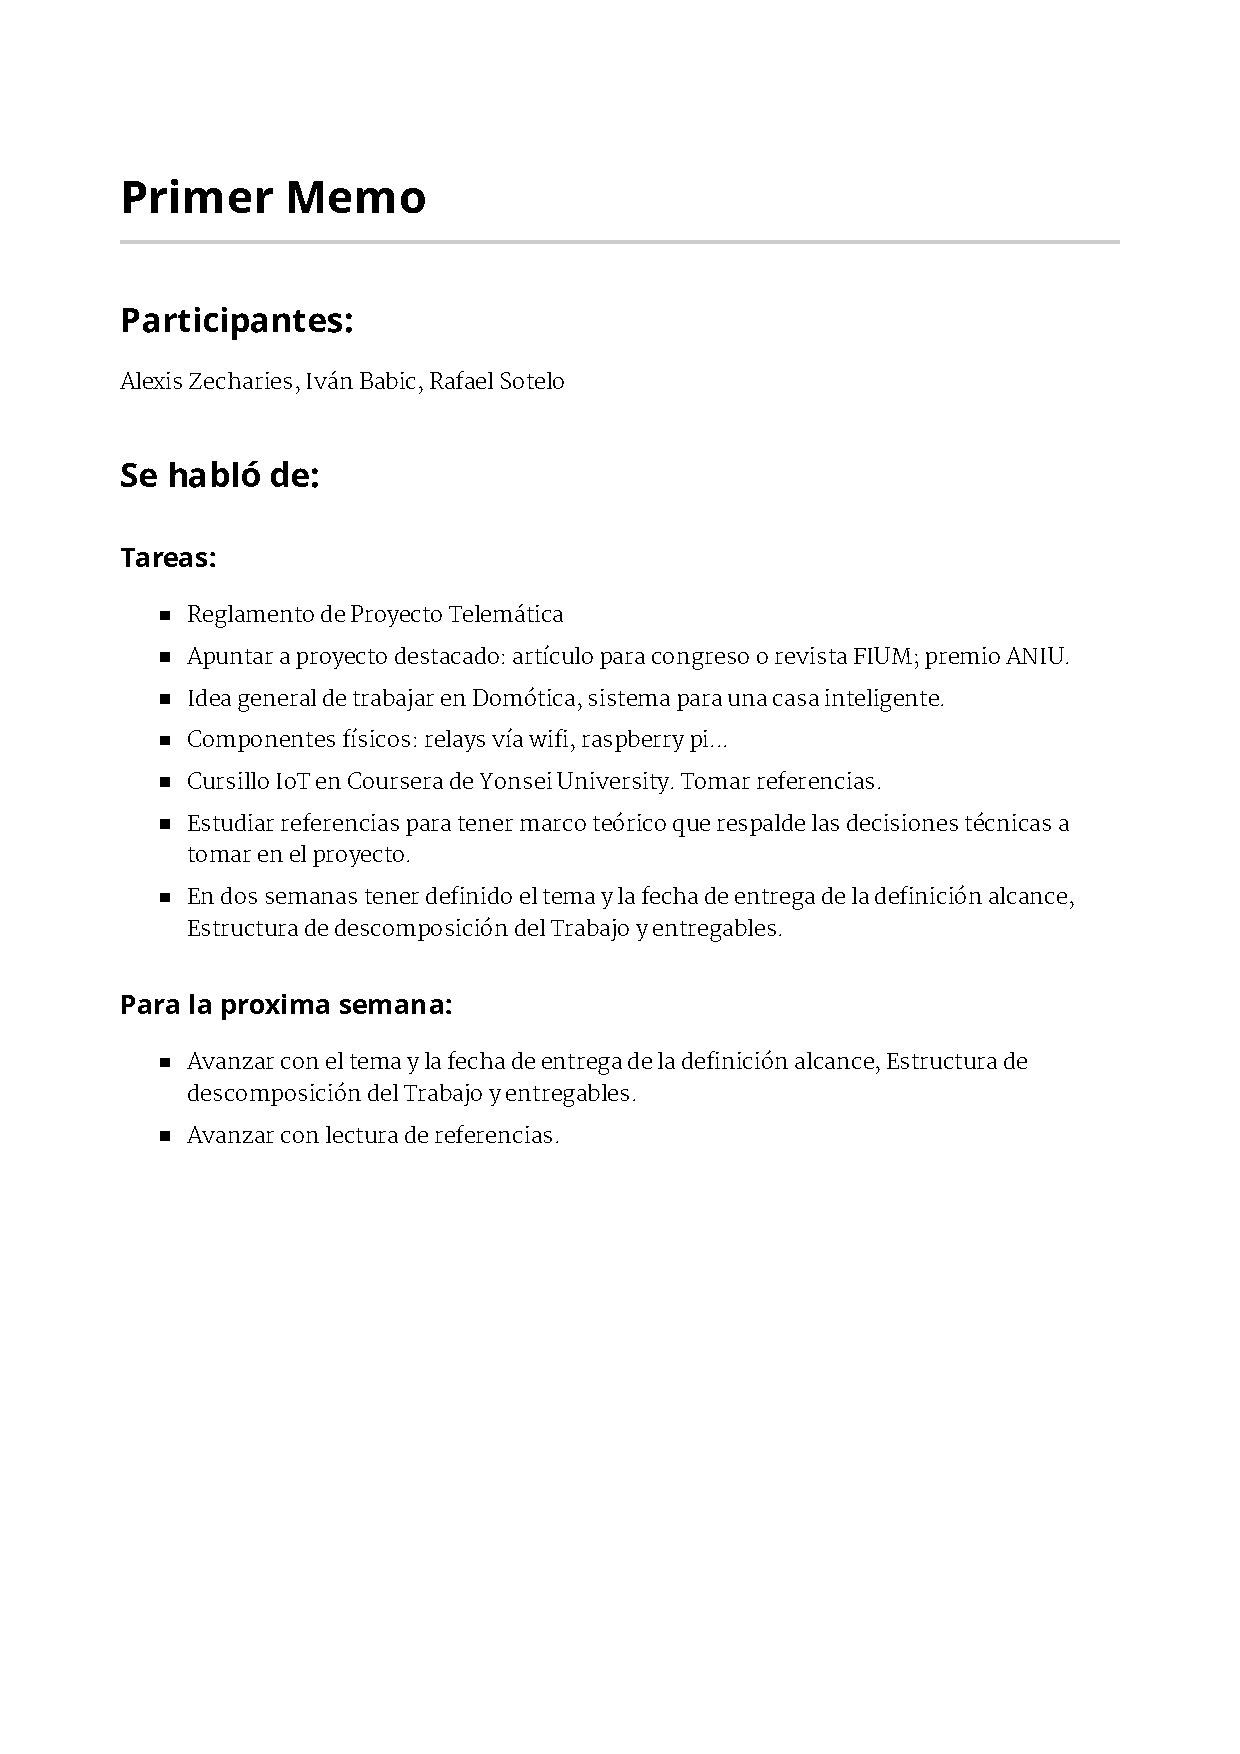
\includepdf[pages=-]{other/memo_1.pdf}
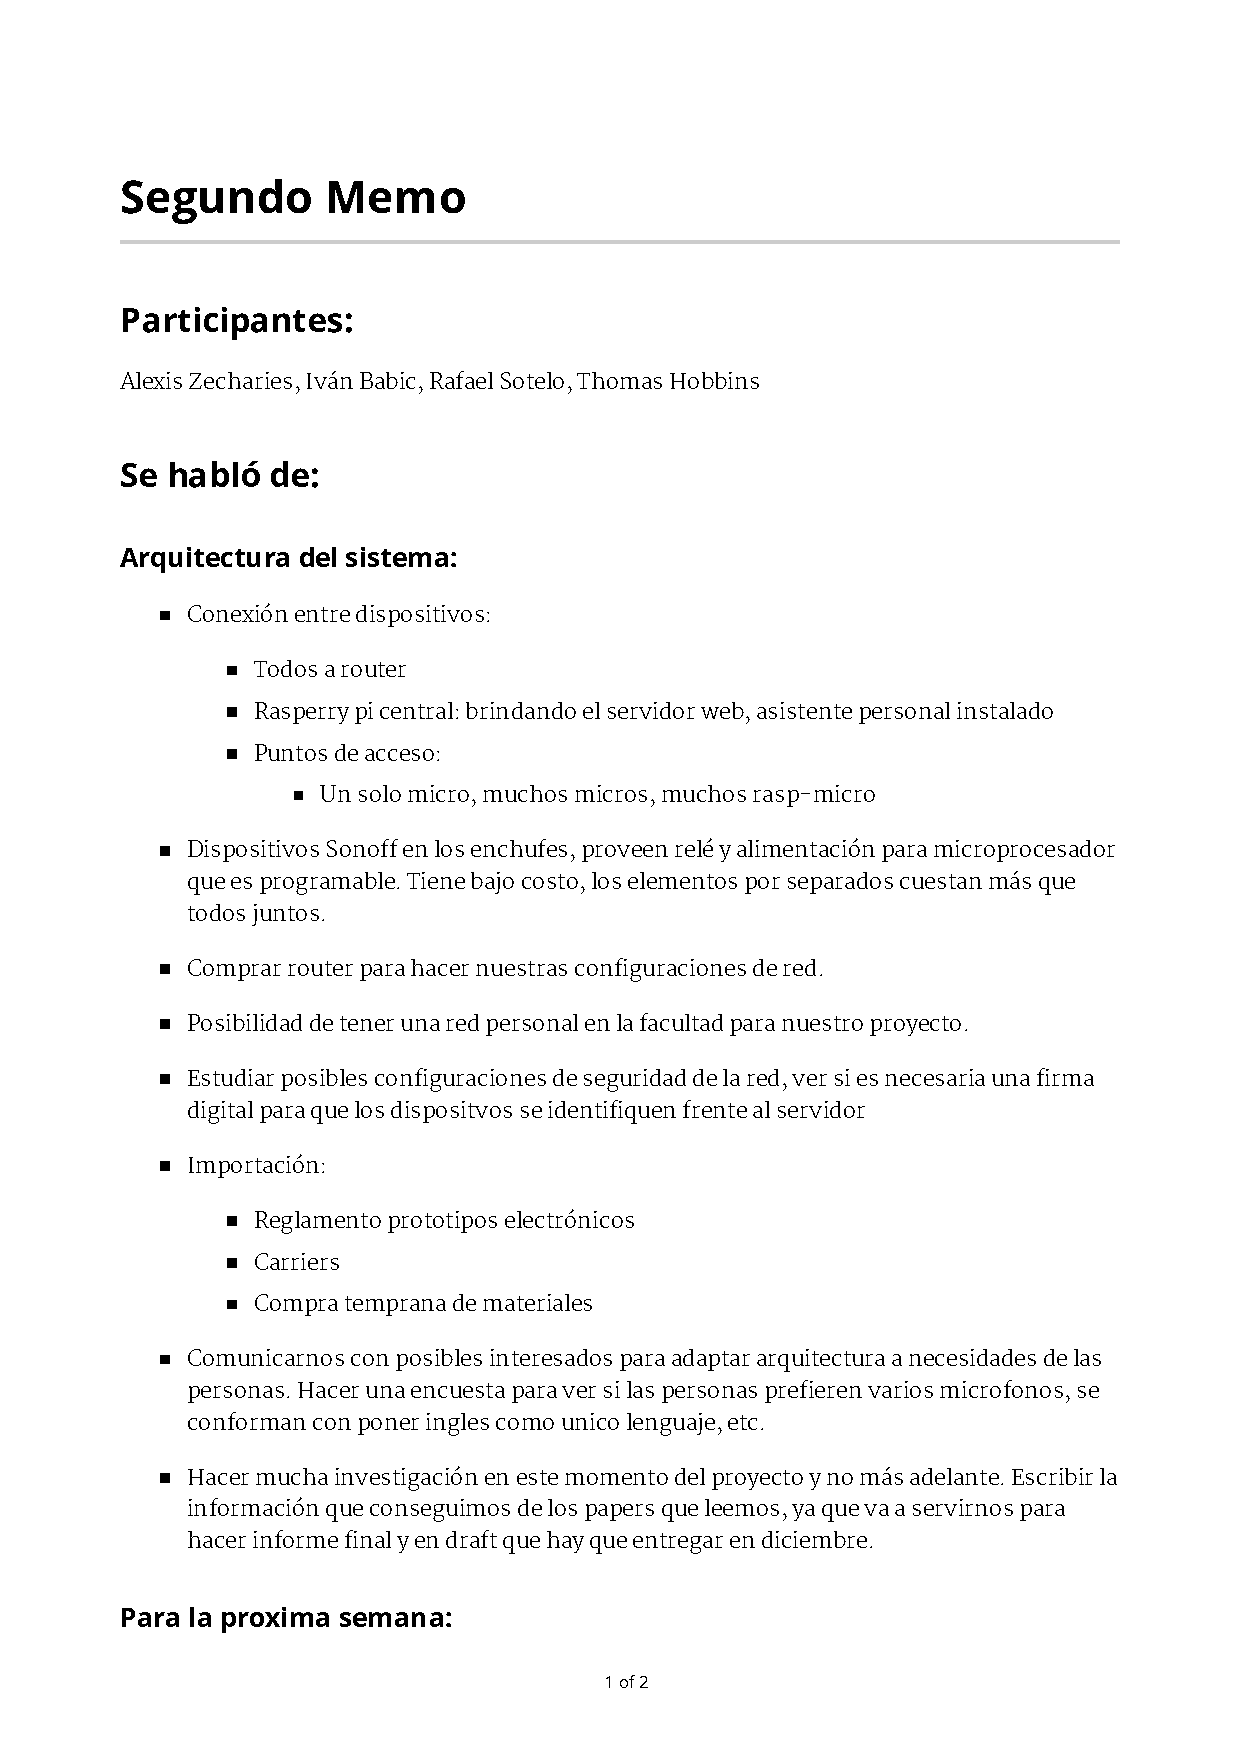
\includepdf[pages=-]{other/memo_2.pdf}
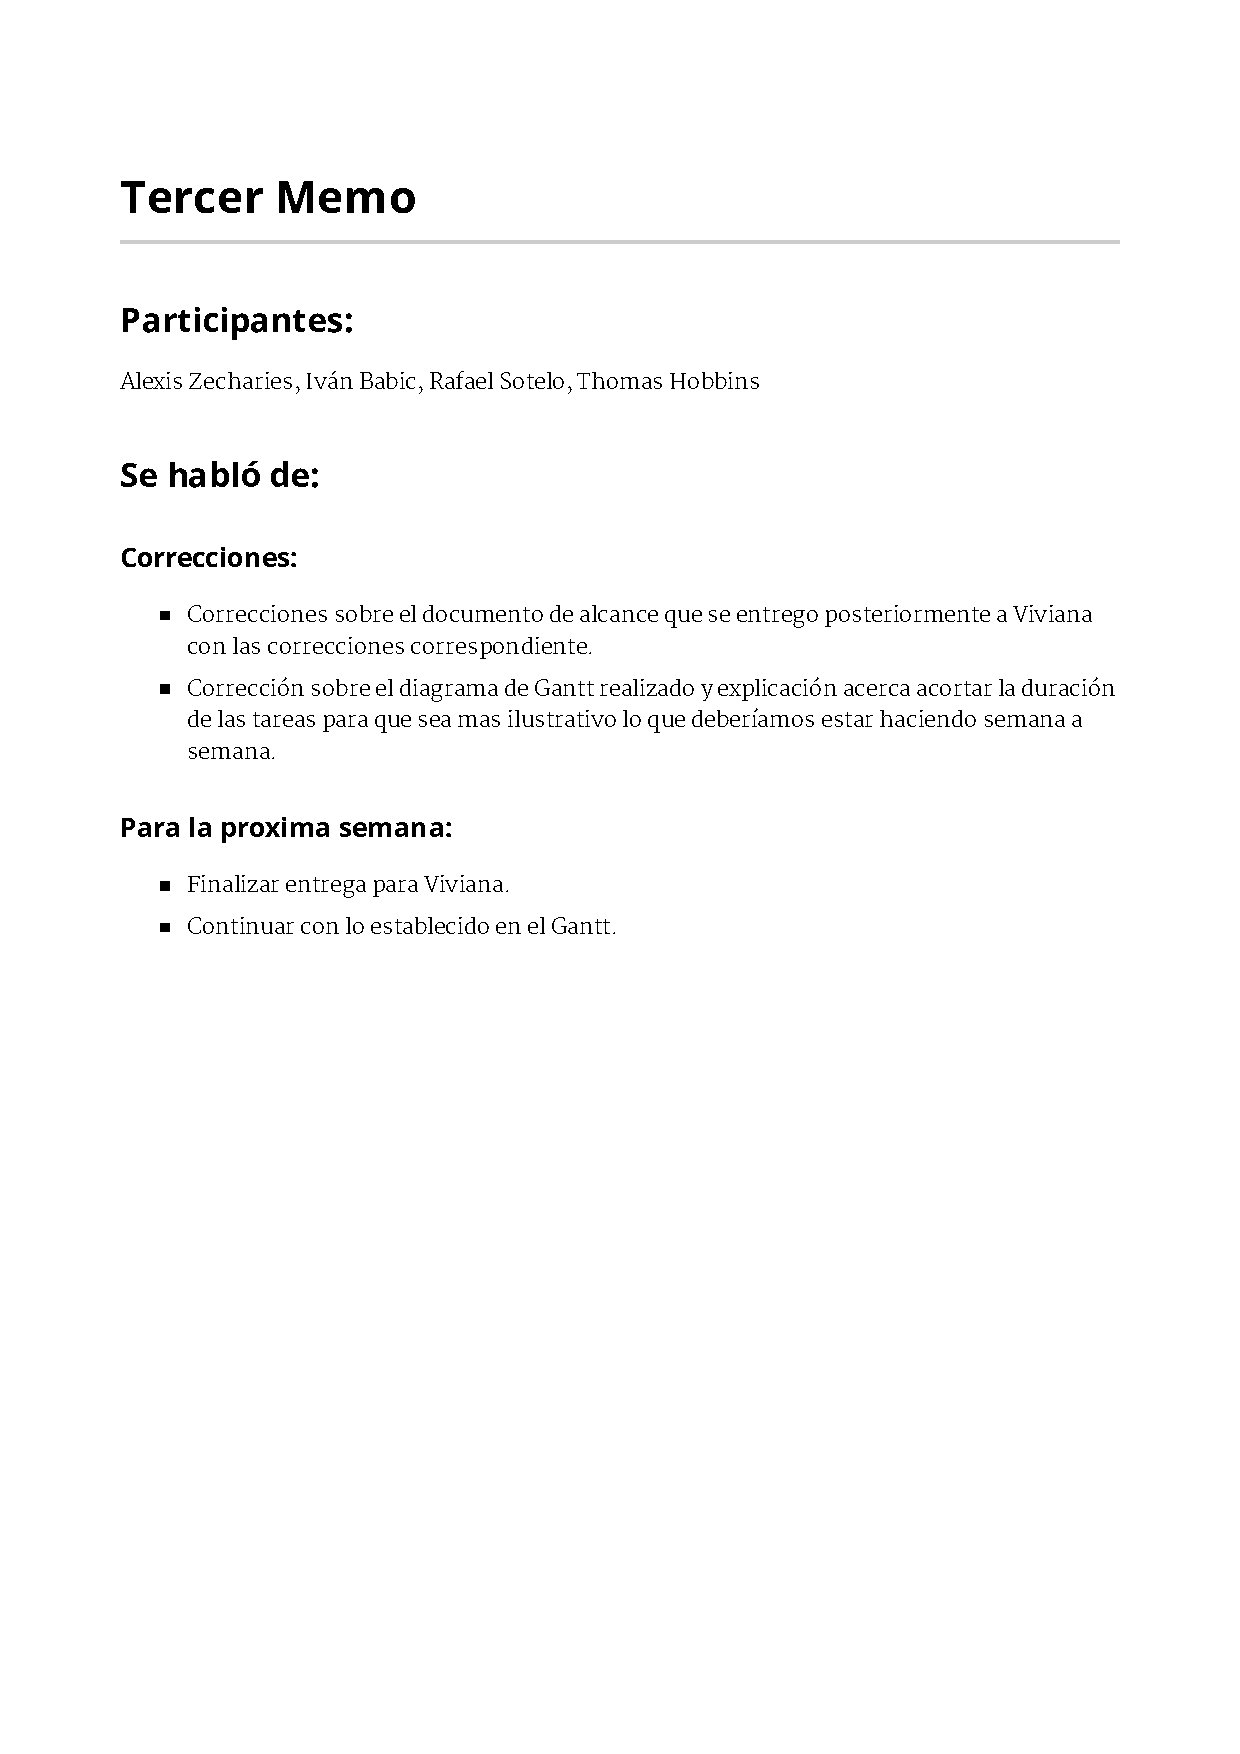
\includepdf[pages=-]{other/memo_3.pdf}
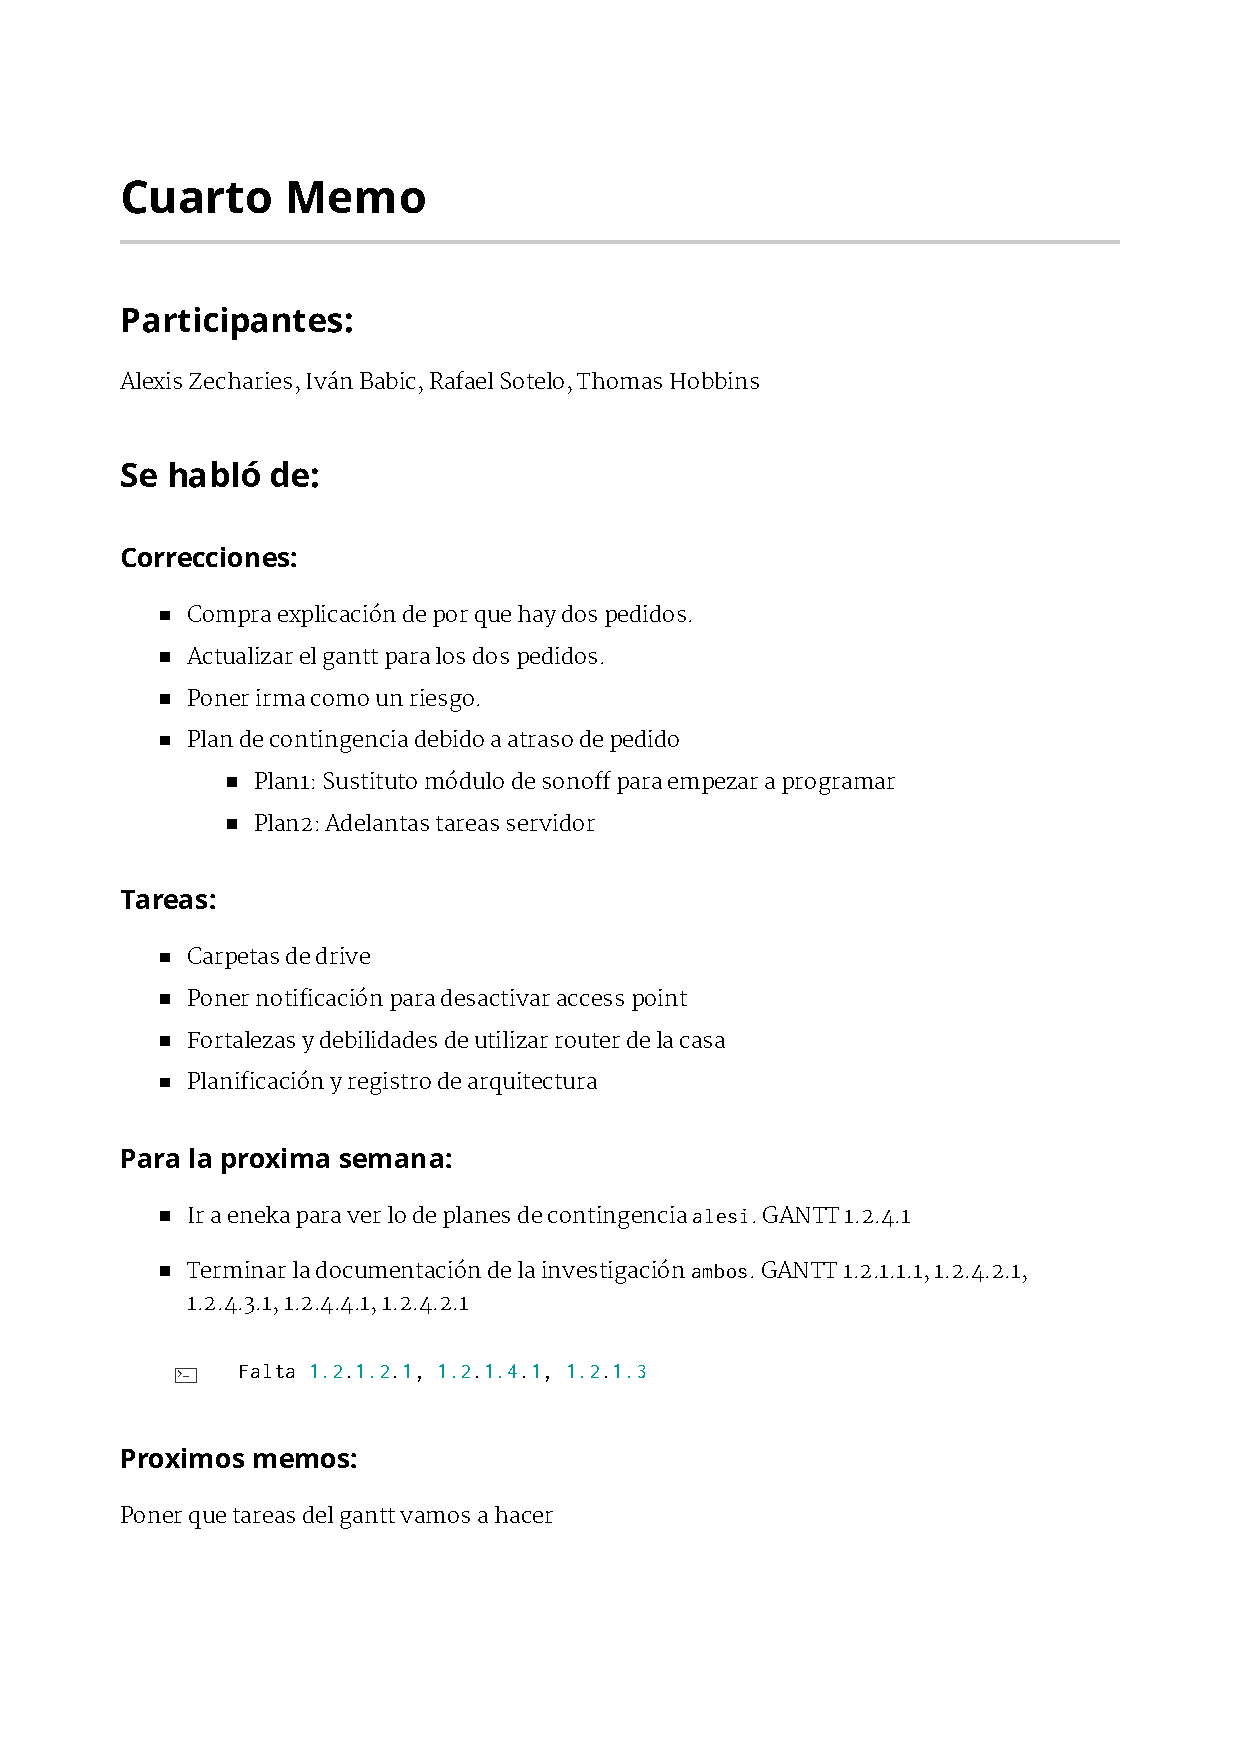
\includepdf[pages=-]{other/memo_4.pdf}
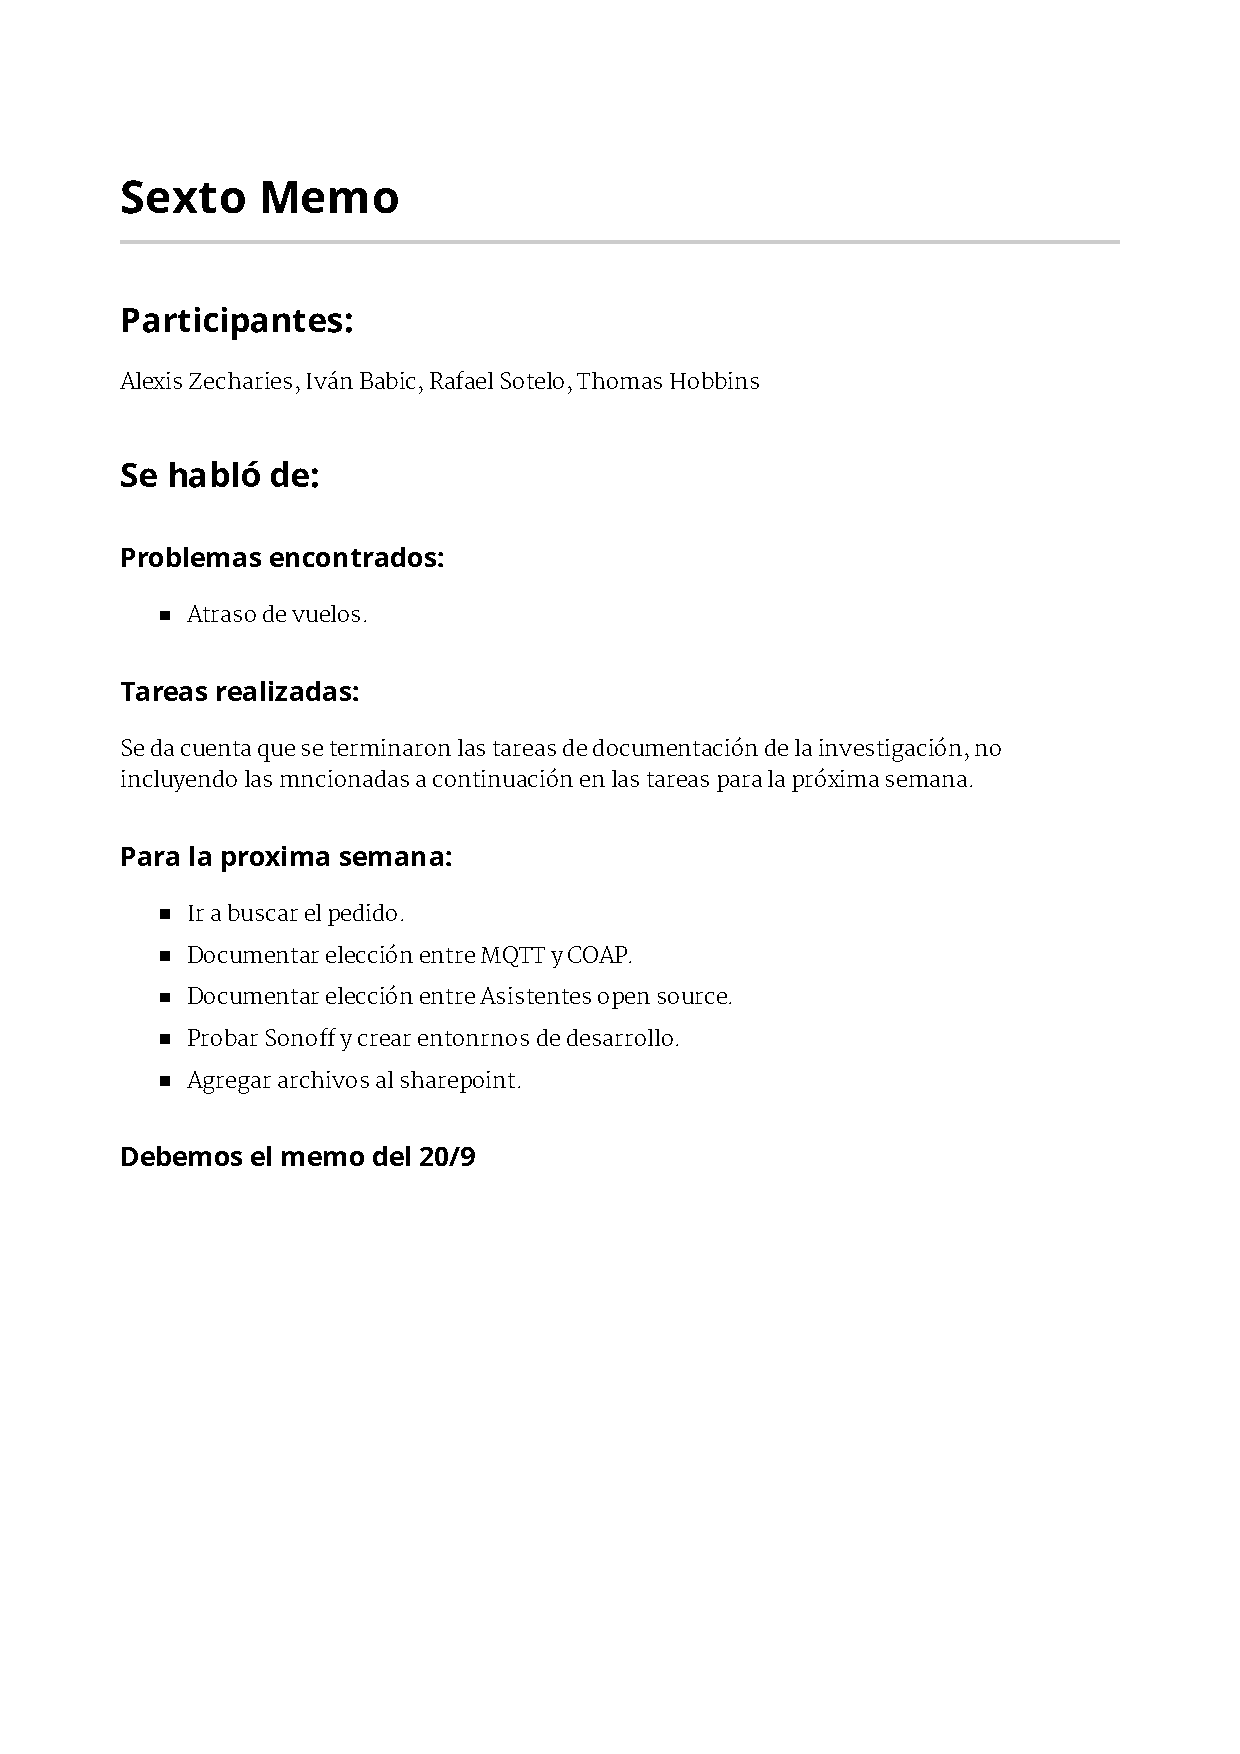
\includepdf[pages=-]{other/memo_6.pdf}
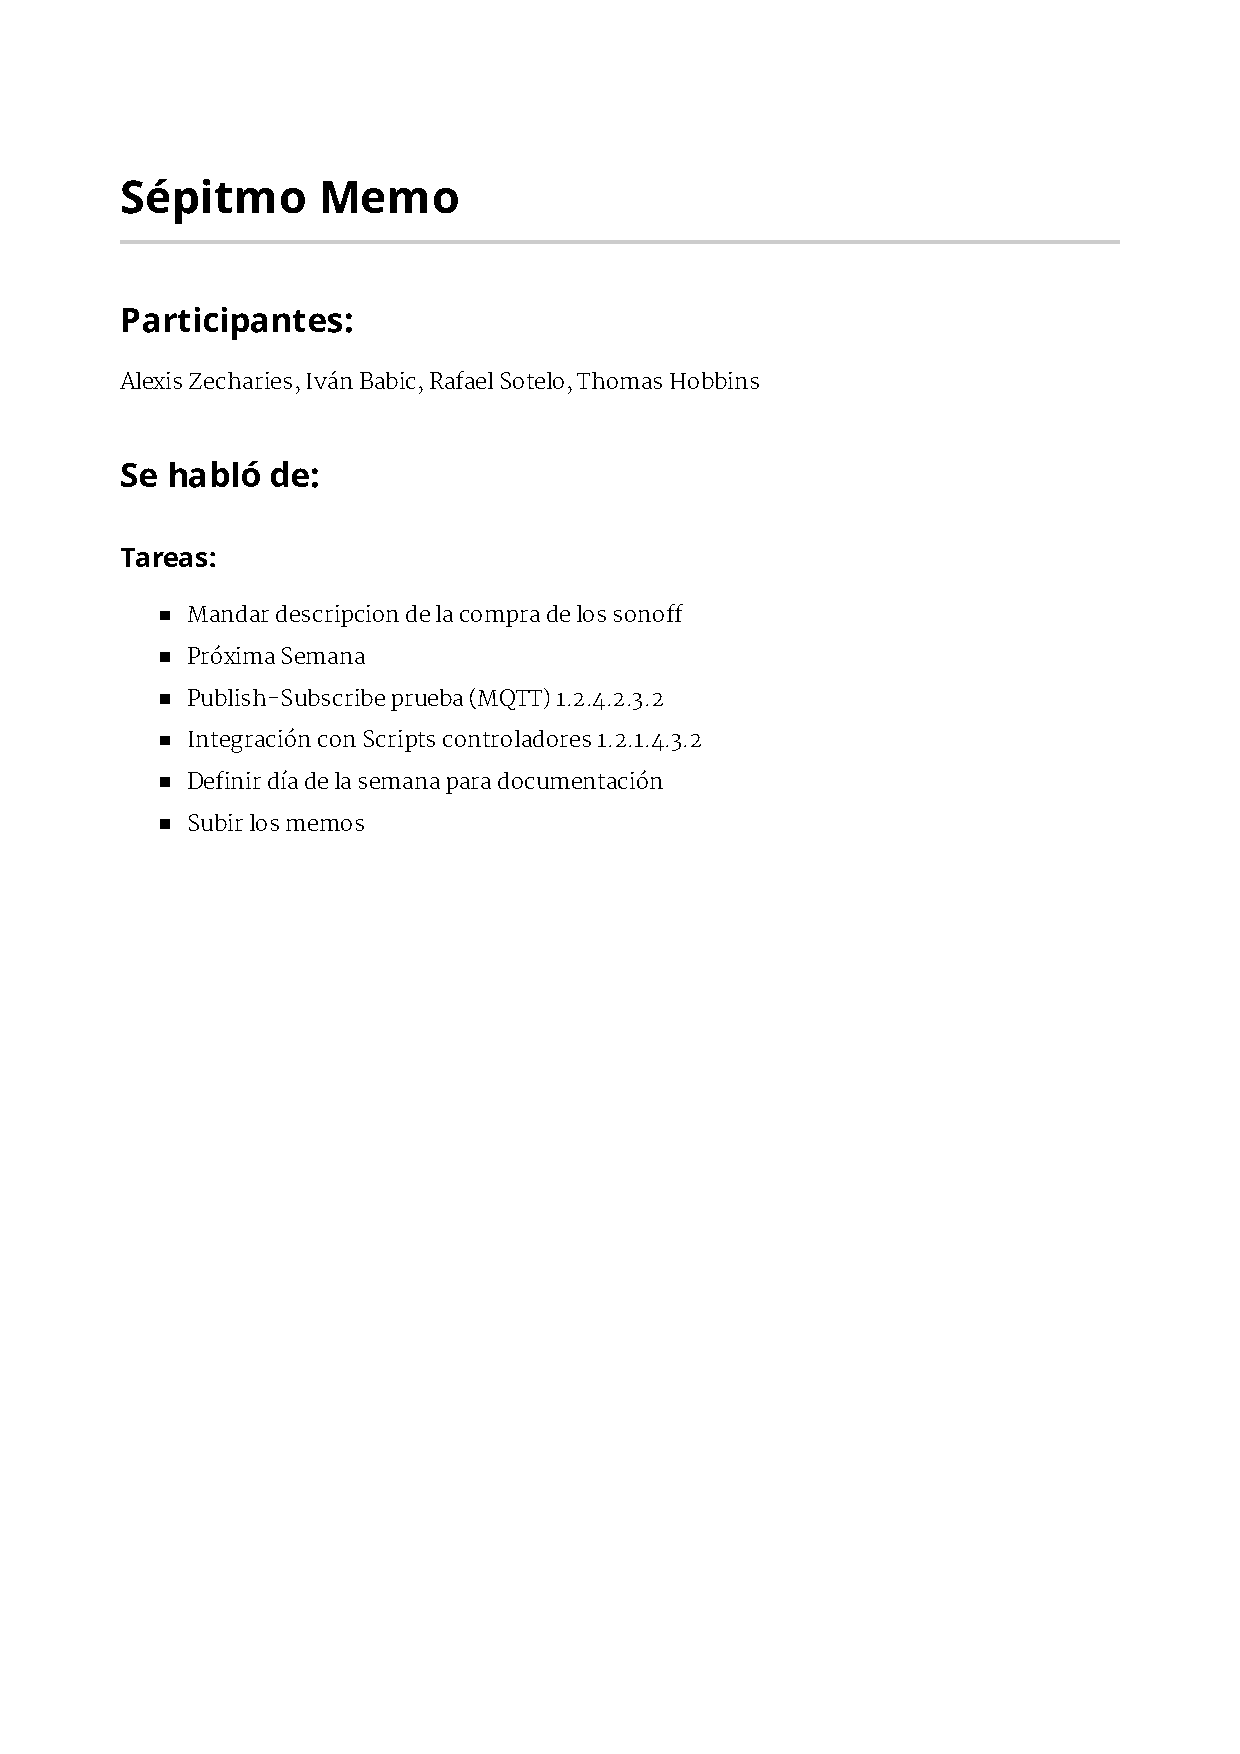
\includepdf[pages=-]{other/memo_7.pdf}
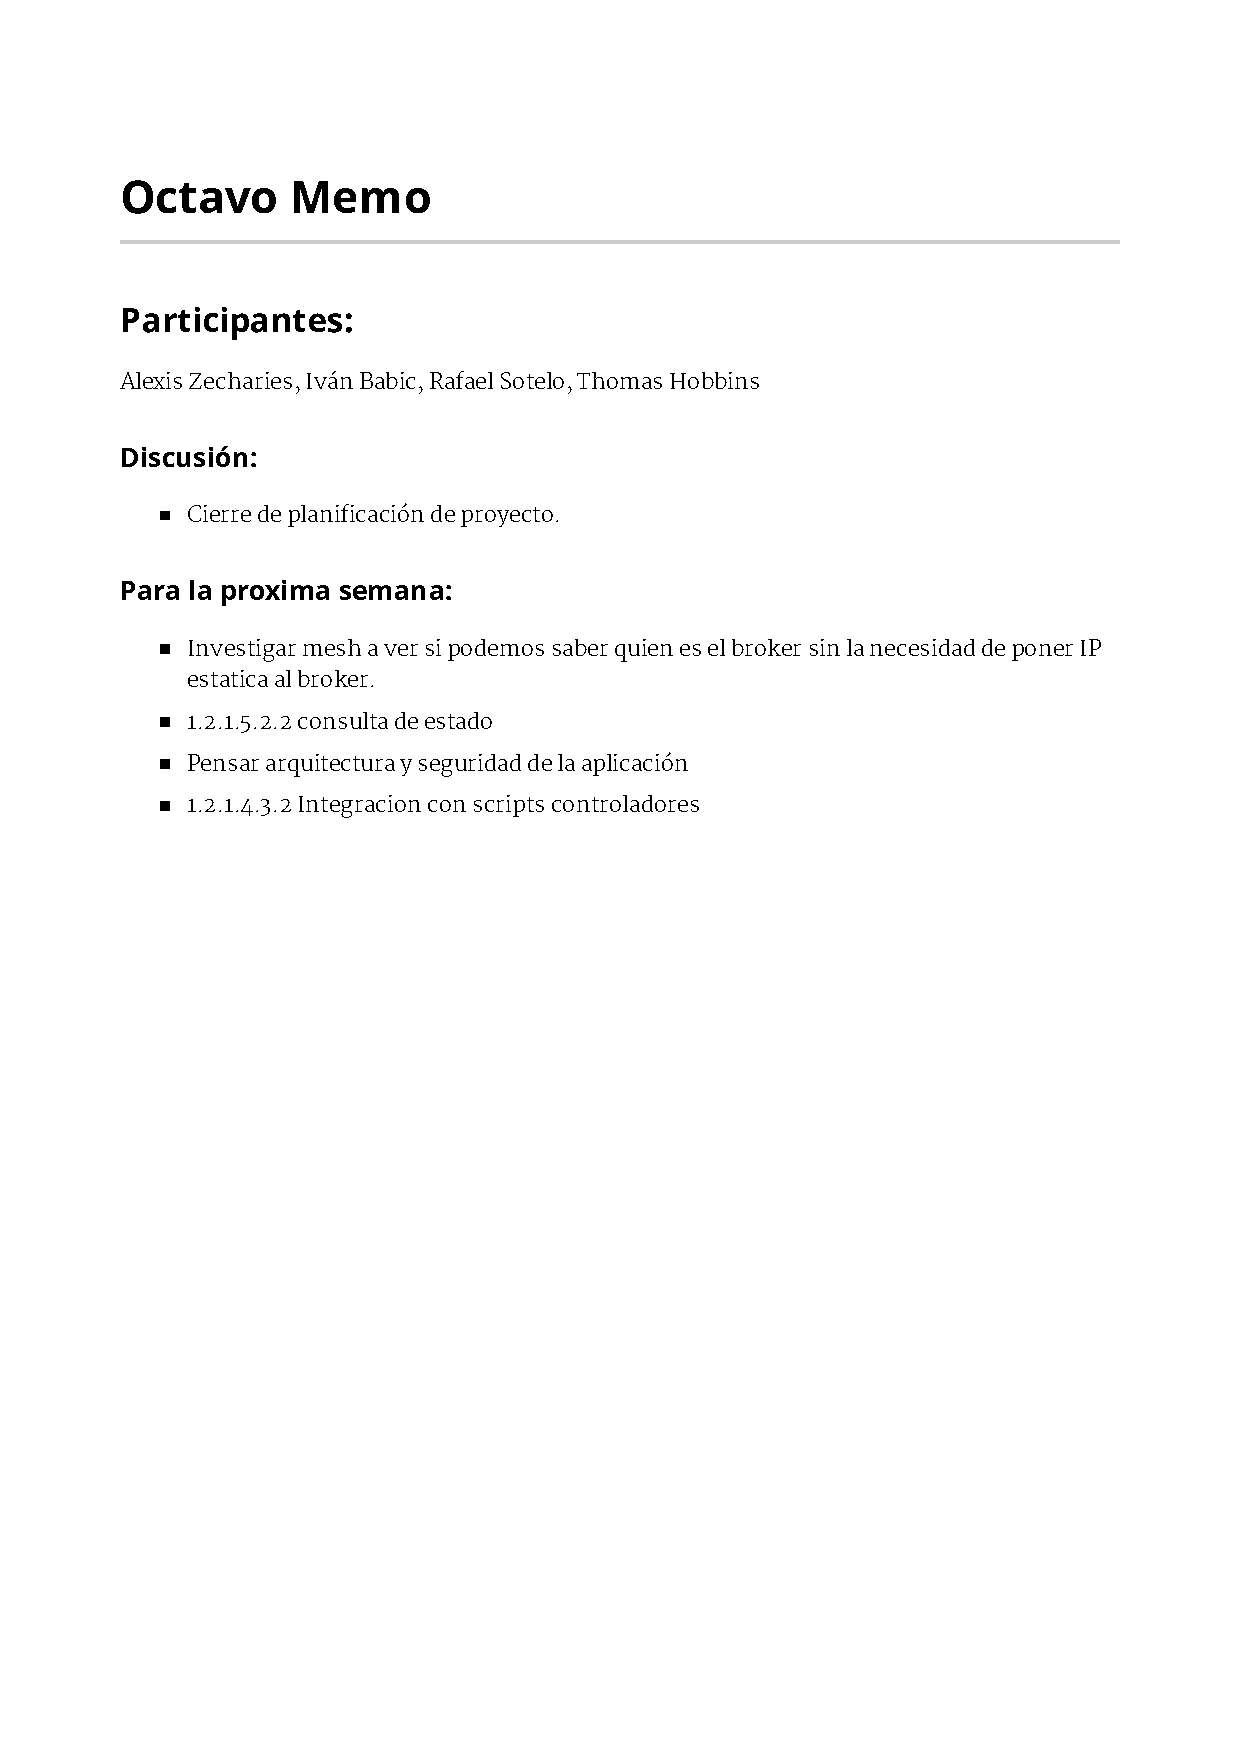
\includepdf[pages=-]{other/memo_8.pdf}
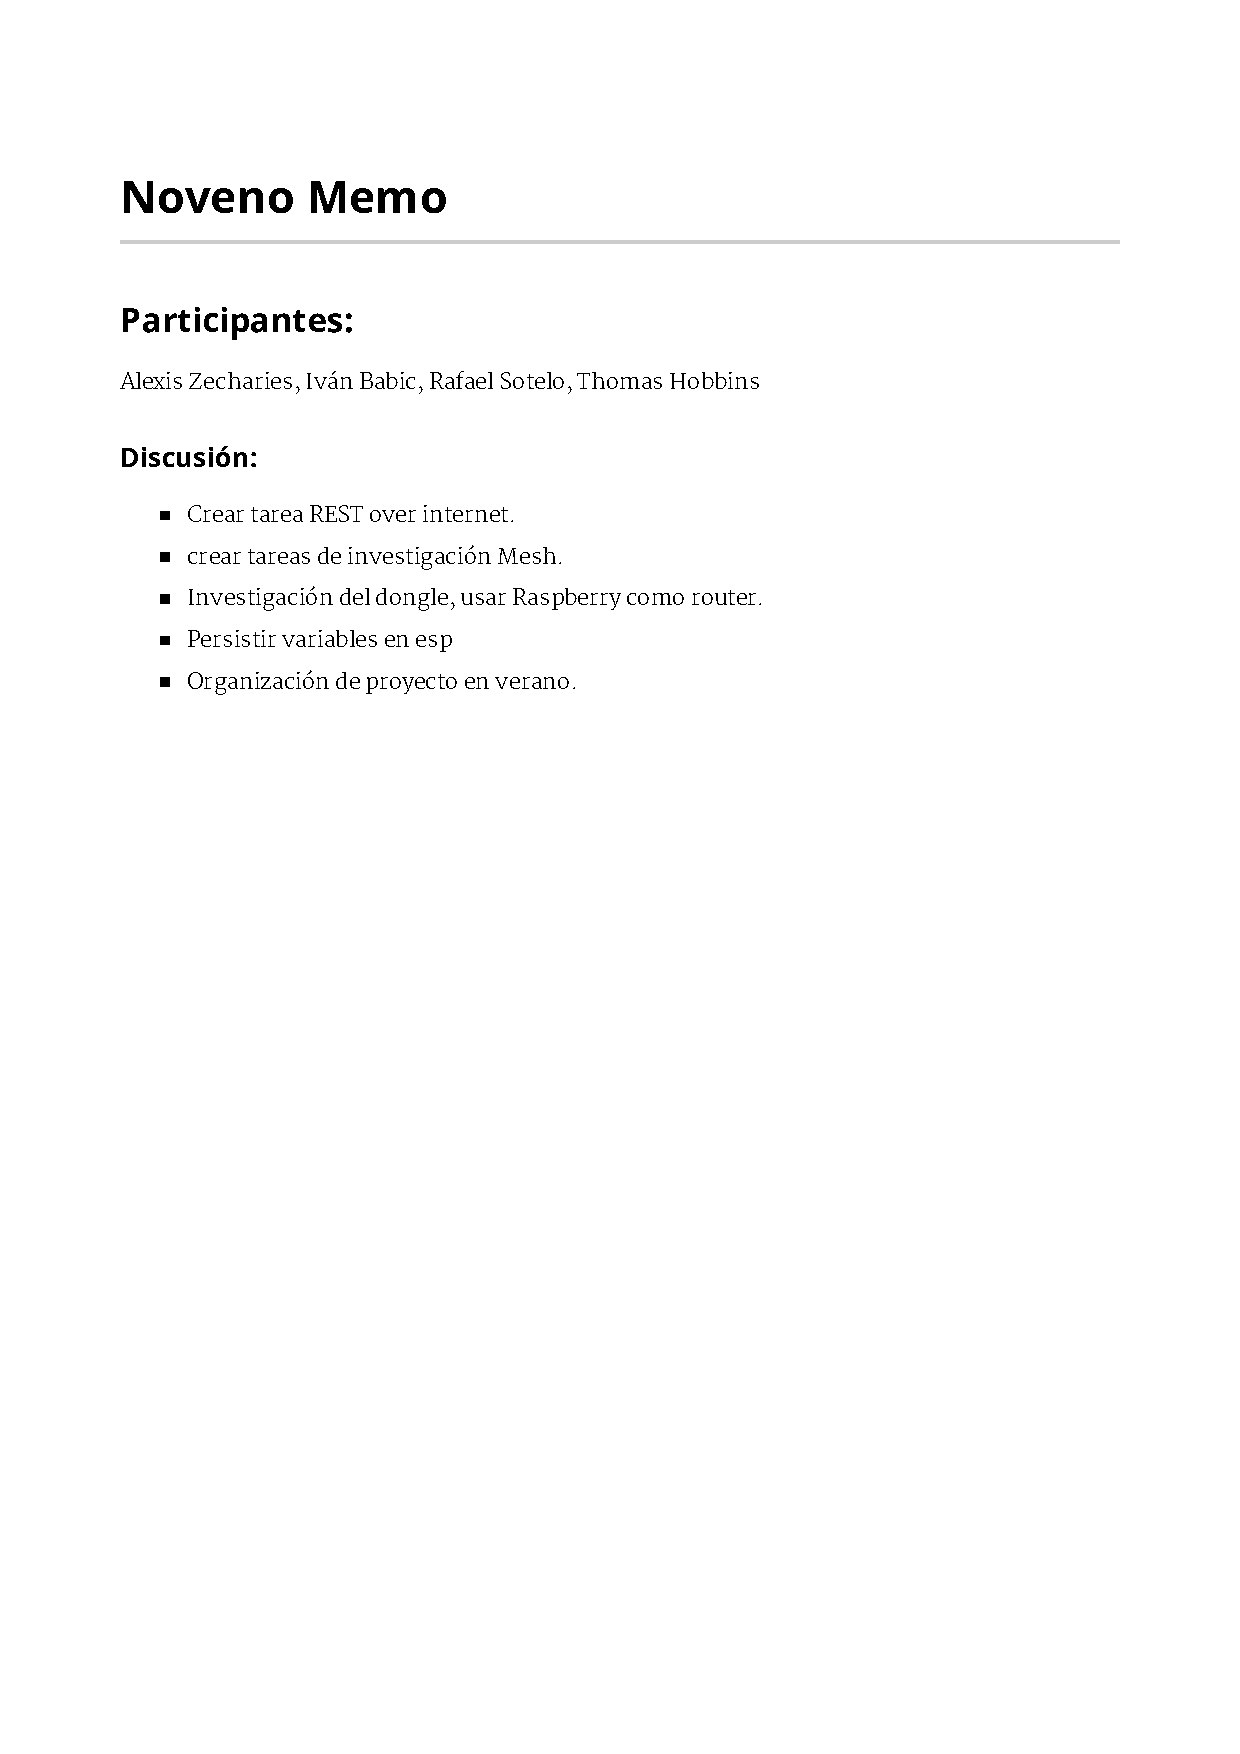
\includepdf[pages=-]{other/memo_9.pdf}

\section{Justificación de avance de 50\%}

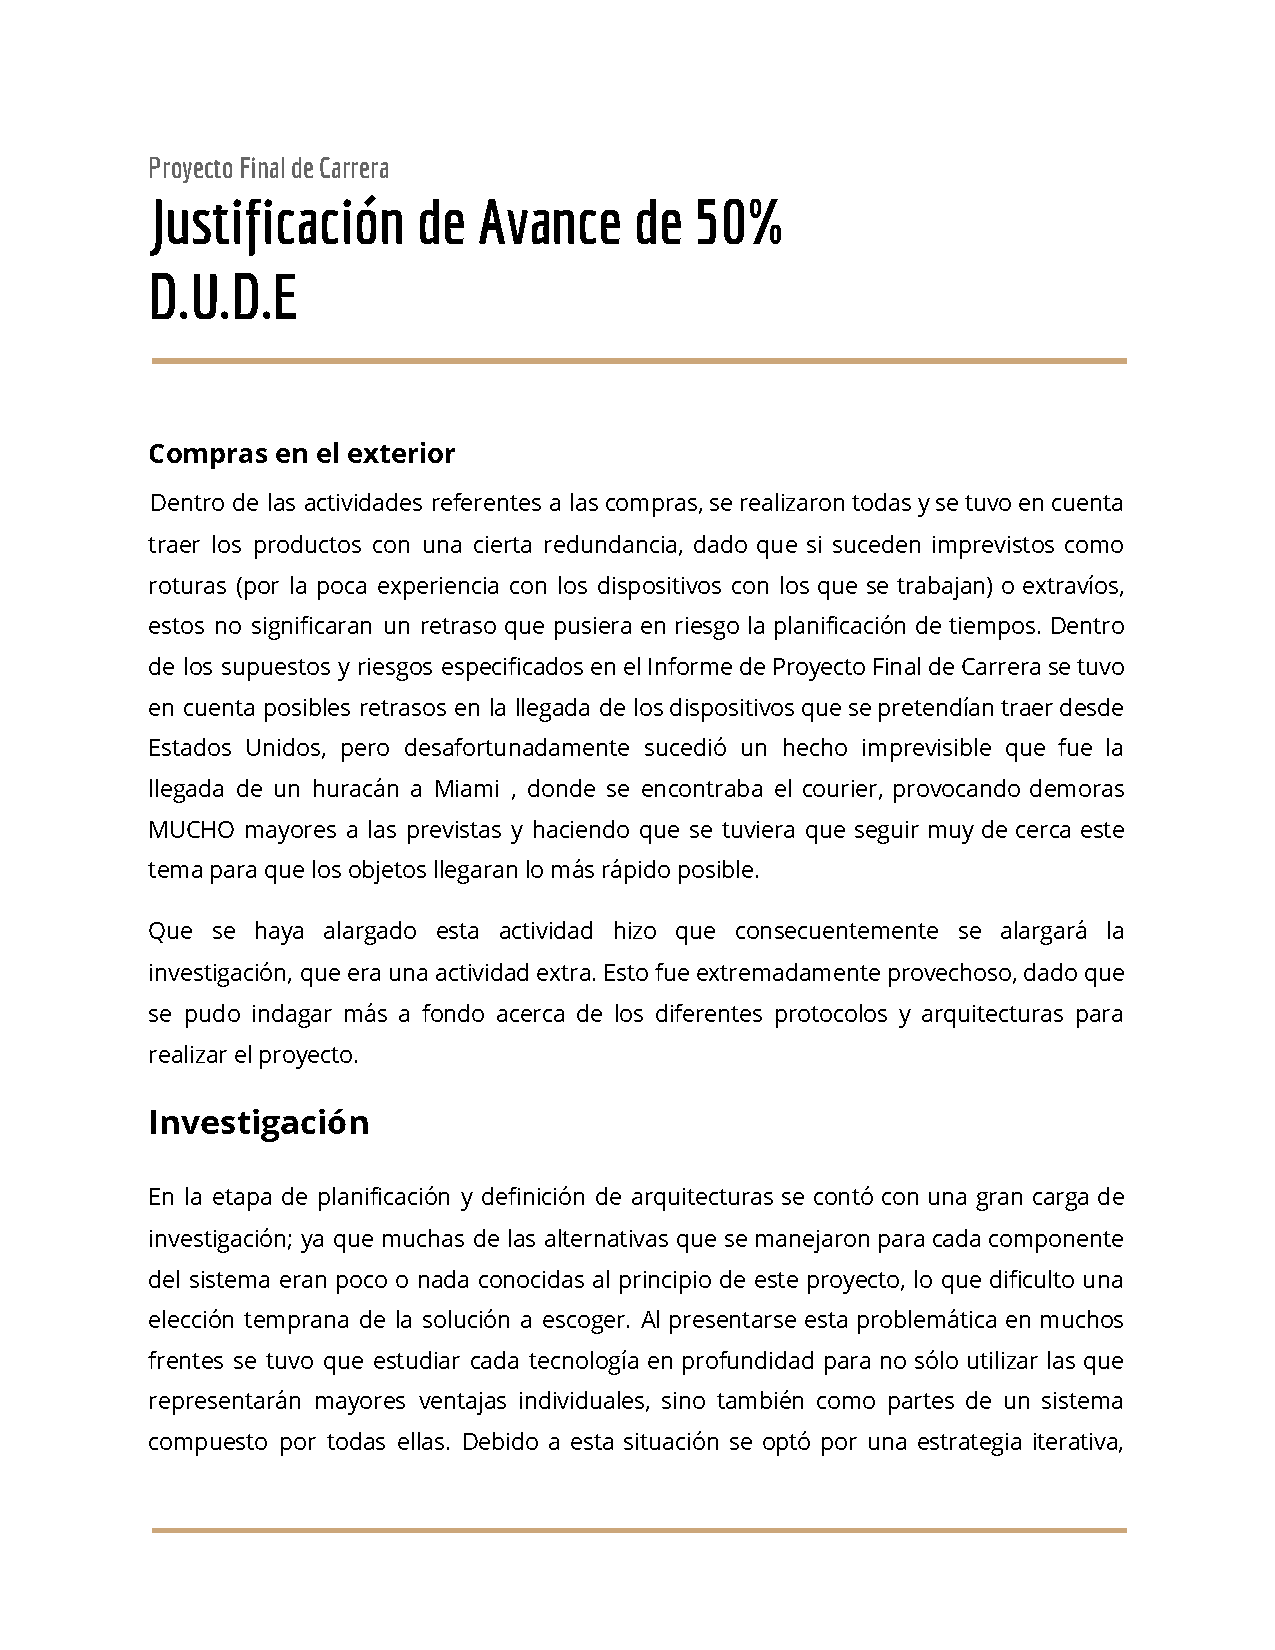
\includepdf[pages=-]{other/justificacion-50.pdf}



\chapter{Código Fuente} \label{anexo-codigo-fuente}


\section{Sonoff} \label{anexo-sonoff}

\subsection{main.cpp} \label{anexo-esp-main}

\lstinputlisting[language=C++]{/Users/IvanBabic/Tesis/esp_mesh/src/main.cpp}

\subsection{credentials.h.j2} \label{anexo-credentials}

\lstinputlisting[language=C++]{/Users/IvanBabic/Tesis/esp_mesh/src/credentials.h.j2}

\subsection{platformio.ini}

\lstinputlisting[language=C++]{/Users/IvanBabic/Tesis/esp_mesh/platformio.ini}


\section{Raspberry Pi} \label{anexo-rpi}

\subsection{mosquitto.conf} \label{anexo-mosquitto.conf}

\lstinputlisting[language=bash]{/Users/IvanBabic/Tesis/MQTT_Server/mosquitto/mosquitto.conf}

\subsection{api.py} \label{api.py}

\lstinputlisting[language=Python]{/Users/IvanBabic/Tesis/MQTT_Server/flask-mqtt/api.py}

\subsection{mongo\_db\_utils.py} \label{anexo-falsk-mongo}

\lstinputlisting[language=Python]{/Users/IvanBabic/Tesis/MQTT_Server/flask-mqtt/mongo_db_utils.py}

\subsection{device\_template.json} \label{anexo-device-template}

\lstinputlisting[language=Python]{/Users/IvanBabic/Tesis/MQTT_Server/flask-mqtt/device_template.json}



\section{Aplicación Web} \label{anexo-app-web}

\subsection{index.js} \label{anexo-index.js}

\lstinputlisting[language=JavaScript]{/Users/IvanBabic/Tesis/dude_web_app/src/index.js}

\subsection{App.js} \label{anexo-app.js}

\lstinputlisting[language=JavaScript]{/Users/IvanBabic/Tesis/dude_web_app/src/App.js}

\subsection{LightControlConsole.js} \label{anexo-lightcontrolconsole.js}

\lstinputlisting[language=JavaScript]{/Users/IvanBabic/Tesis/dude_web_app/src/LightControlConsole.js}




